\documentclass[a4paper,12pt]{report}
\usepackage[utf8]{vietnam}
\usepackage{graphicx}
\usepackage{fancybox}
\usepackage{longtable}
\usepackage{listings}
\usepackage{relsize}
\usepackage{cases} 
\usepackage[left=3cm, right=2.00cm, top=2.00cm, bottom=2.00cm]{geometry}
\lstset{
   %keywords={break,case,catch,continue,else,elseif,end,for,function,
   %   global,if,otherwise,persistent,return,switch,try,while},
   basicstyle=\ttfamily \fontsize{12}{15}\selectfont,   
	% numbers=left,
   frame=lrtb,
tabsize=2
}
\usepackage{hyperref}
\usepackage{float}
\hypersetup{
    colorlinks,
    citecolor=black,
    filecolor=black,
    linkcolor=black,
    urlcolor=black
}
\usepackage[nottoc]{tocbibind}
\usepackage[english]{babel}
\usepackage{indentfirst}
\addto\captionsenglish{%
 \renewcommand\chaptername{Phần}
 \renewcommand{\contentsname}{Mục lục} 
 \renewcommand{\listtablename}{Danh sách bảng}
 \renewcommand{\listfigurename}{Danh sách hình vẽ}
 \renewcommand{\tablename}{Bảng}
 \renewcommand{\figurename}{Hình}
}
\begin{document}
\thispagestyle{empty}
\thisfancypage{
\setlength{\fboxrule}{1pt}
\doublebox}{}
\begin{center}
{\fontsize{16}{19}\fontfamily{cmr}\selectfont TRƯỜNG ĐẠI HỌC BÁCH KHOA HÀ NỘI\\
VIỆN CÔNG NGHỆ THÔNG TIN VÀ TRUYỀN THÔNG}\\
\textbf{------------*******---------------}\\[1cm]

\includegraphics[scale=0.13]{hust.jpg}\\[1.3cm]

{\fontsize{32}{43}\fontfamily{cmr}\selectfont BÁO CÁO}\\[0.1cm]
{\fontsize{38}{45}\fontfamily{cmr}\fontseries{b}\selectfont MÔN HỌC}\\[0.2cm]
{\fontsize{19}{20}\fontfamily{phv}\selectfont Học máy }\\[0.2cm]
{\fontsize{13}{20}\fontfamily{cmr}\selectfont Đề tài: So sánh thử nghiệm các phương pháp học máy\\ cho bài toán phân loại ảnh.
}\\[2.5cm]
\end{center}
\hspace{1cm}\fontsize{14}{16}\fontfamily{cmr}\selectfont \textbf{Nhóm sinh viên thực hiện:}

\begin{longtable}{l c c}

Họ và tên & MSSV  & Lớp\\
Nguyễn Tuấn Đạt & 20130856 & CNTT2.02-K58 \\
Vũ Minh Đức & 20131081 & CNTT2.03-K58 \\
Nguyễn Ngọc Huyền & 20131821 & CNTT2.03-K58 \\
Đặng Quang Trung & 20134145 & CNTT2.02-K58 \\
Phan Anh Tú & 20134501 & CNTT2.01-K58 \\
\end{longtable}

\hspace{1cm}\fontsize{14}{16}\fontfamily{cmr}\selectfont \textbf{Giáo viên hướng dẫn: }TS.Thân Quang Khoát \\[1.5cm]
\begin{center}
\fontsize{16}{19}\fontfamily{cmr}\selectfont Hà Nội 12--2016

\end{center}
\newpage
\pdfbookmark{\contentsname}{toc}
\tableofcontents
\chapter*{Lời cảm ơn}
Chúng em xin chân thành cảm ơn Thầy giáo, TS. Thân Quang Khoát đã tận tình giảng dạy, hướng dẫn chúng em thực hiện đề tài này. Trong quá trình thực hiện, đề tài của chúng em không tránh khỏi những hạn chế, thiếu sót, chúng em rất mong nhận được những ý kiến đánh giá, nhận xét của Thầy để đề tài này có thể được hoàn thiện hơn.
\phantomsection
\addcontentsline{toc}{chapter}{Lời cảm ơn}

\listoffigures
\chapter*{Mở đầu}
\addcontentsline{toc}{chapter}{Mở đầu}
Học máy là lập trình cho máy tính để tối ưu hóa các tiêu chí hiệu suất, sử dụng dữ liệu mẫu hoặc các kinh nghiệm từ quá khứ. Hiện nay đã có nhiều ứng dụng của Học máy thành công trên nhiều mảng khác nhau: Các hệ thống đã được đưa vào thương mại hóa giải quyết vấn đề nhận diện giọng nói và chữ viết; Các công ty bán lẻ phân tích dữ liệu bán hàng từ quá khứ để học hành vi của khách hàng, để từ đó tăng cường, cải thiện việc quản lý các mối quan hệ với khách hàng; Robot học để tối ưu hành vi, với mục đích là hoàn thành nhiệm vụ với lượng tài nguyên sử dụng nhỏ nhất… \\

Cùng với những thành tựu tiên tiến trong công nghệ về máy tính, chúng ta đã có khả năng lưu trữ và xử lý lượng lớn dữ liệu, cũng như truy cập chúng từ khoảng cách lớn về địa lý thông qua mạng máy tính. Lượng dữ liệu được lưu trữ đó chỉ trở nên hữu dụng khi nó được phân tích và đưa về các thông tin ta có thể sử dụng được, nhờ các ứng dụng về xử lý dữ liệu lớn của Học máy. Học máy đang là một lĩnh vực đầy tiềm năng nghiên cứu, mang lại nhiều lợi ích mang tính đột phá, có ý nghĩa lớn về cả mặt lý thuyết và ứng dụng. \\

Đề tài của chúng em trình bày những tìm hiểu về một khía cạnh của Học máy: Phân loại hình ảnh. Trong đó, chúng em sử dụng các phương pháp đặc trưng trong học máy để giải quyết bài toán phân loại hình ảnh với bộ dữ liệu cho trước, từ đó so sánh, đánh giá và đưa ra kết luận cho bài toán. 
\chapter{Mô tả bài toán}
\section{Giới thiệu bài toán}
Với bài toán phân loại hình ảnh, một bức ảnh được phân loại dựa theo nội dung về mặt hình ảnh. Đây là bài toán học có giám sát: Toàn bộ các bức ảnh đều được gán nhãn. \\

Mục đích của quá trình phân loại là đưa ra nhãn lớp của hình ảnh đưa vào. Ta xét với bộ dữ liệu chứa các ảnh kích cỡ 32x32 pixel, với 3 kênh màu: Đỏ, xanh lá cây, xanh dương. Mỗi hình ảnh được dãn ra thành một vector cột nhiều chiều, ta có thể coi mỗi hình ảnh như một điểm trong không gian 3072 chiều (32x32x3 pixel). Ta có thể coi toàn bộ tập dữ liệu là tập các điểm được gán nhãn. 

\begin{itemize}
\item Đầu vào: Bộ dữ liệu ảnh training đã được mã hóa và gán nhãn
\end{itemize} 
\begin{itemize}
\item Đầu ra: Với một mô hình đã học và đưa vào thử nghiệm trên tập test, đưa ra nhãn lớp tương ứng với hình ảnh đầu vào, dựa trên kết quả đó để đánh giá phương pháp học máy.
\end{itemize}
\section{Bộ dữ liệu sử dụng}
Bộ dữ liệu CYFAR-10 chứa 60000 hình ảnh màu 32x32 trong 10 nhãn lớp, với 6000 hình ảnh mỗi lớp. Có tổng cộng 50000 hình ảnh học và 10000 hình ảnh để thử nghiệm.\\

Bộ dữ liệu được chia thành 5 batch để học, mỗi batch có 10000 hình ảnh. Bộ thử nghiệm chứa chính xác 1000 bức ảnh từ mỗi lớp. Các batch để học chứa số ảnh còn lại, xếp theo thứ tự ngẫu nhiên, do đó có thể có một vài batch chứa nhiều hình ảnh của một lớp hơn batch khác. Cộng các batch học lại, có chính xác 5000 hình ảnh từ mỗi lớp.
\section{Các phương pháp thử nghiệm}
\begin{itemize}
\item K-NN: Học dựa trên láng giềng gần nhất
\item Neural Network: Mạng nơ ron
\item Convolutional Neural Networks
\item Support Vector Machine: Máy vector hỗ trợ
\end{itemize}
\chapter{Các phương pháp sử dụng và kết quả thực nghiệm}
\section{KNN}
\subsection{Cơ sở lý thuyết}
\begin{itemize}
\item Giai đoạn học
\begin{itemize}
\item KNN - K nearest neighbors : là một phương pháp học máy dựa trên việc lưu lại các các ví dụ học trong tập dữ liệu training.
\end{itemize}
\item Giai đoạn phân lớp
\begin{itemize}
\item Dùng một hàm để tính độ tương đồng giữa các ví dụ traning đã lưu và dữ liệu từ bộ test. 
\item Lưu lại k ví dụ có độ tương đồng với dữ liệu test nhất, từ đó dự đoán nhãn cho ví dụ test đầu vào theo lớp chiếm số đông trong số các lớp của k láng giềng. 
\end{itemize}
\item Vấn đề cần giải quyết với giải thuật KNN
\begin{itemize}
\item Có nhiều hàm tính độ tương đồng, cần lựa chọn và thử nghiệm để chọn ra hàm tương đồng phù hợp với bộ dữ liệu.
\item Lấy bao nhiêu hàng xóm cho đủ. 
\end{itemize}
\end{itemize}
\subsection{Cài đặt}
\begin{itemize}
\item Biểu diễn dữ liệu: mỗi dữ liệu sẽ được biểu diễn thông qua các vector $x=(x_1,x_2,...,x_n,y)$
\begin{itemize}
\item $x_i$ là các thuộc tính 
\item y là nhãn lớp
\end{itemize}
\item Lựa chọn mô hình
\begin{itemize}
\item Hàm tính độ tương đồng  :D(x,y)= $\sum_{i=1}^n(\left\|x_i - y_i\right\|)$
\begin{figure}[H]
\centering
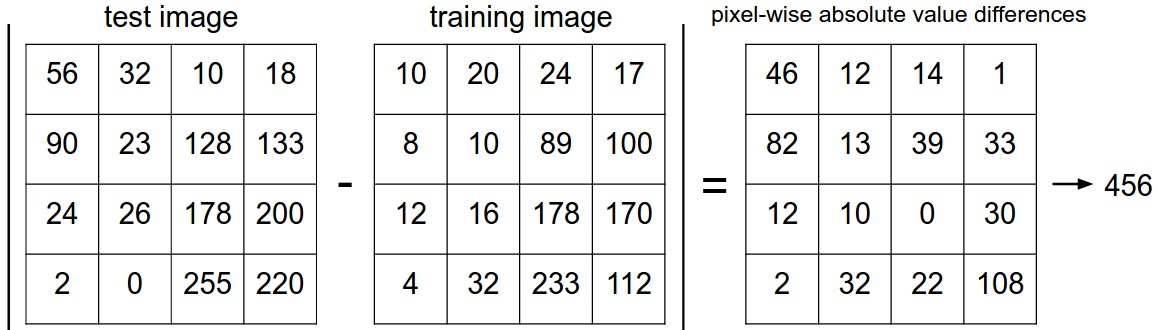
\includegraphics[scale=0.4]{dknn.jpeg}
\caption{Function distance KNN}
\label{fig:knn}
\end{figure}
\item Lựa chọn k:
\begin{figure}[H]
\centering
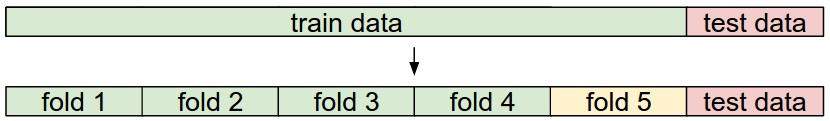
\includegraphics[scale=0.4]{crossval.jpeg}
\caption{Split data}
\label{fig:splitdata}
\end{figure}
\begin{itemize}
\item Bước đầu, dữ liệu được chia ra thành 2 phần train và test
\item Tiếp theo từ tập train, chia dữ thành 5 fold, lấy 4 fold cho việc học, 1 fold dùng validation
\item Thử cho các giá trị  $k={3,4,5,6,7}$, lựa chọn các giá trị tốt nhất
\end{itemize}
\end{itemize}
\end{itemize}
(ghi chú: cần nêu rõ cấu trúc mã nguồn, chương trình, vai trò của các lớp và các phương thức chính)

\subsection{Kết quả}
\begin{itemize}
\item K thu được là 7
\item Kết quả $\approx 11\% $
\begin{center}
\begin{longtable}{lccccccccl}
\caption{\textbf{Bảng mô tả kết quả KNN}}
\endfirsthead
\endhead
\hline
0       &    1   &   2    &     3    &    4    &    5    &    6    &     7   &    8    &    9  \\
\hline
$40\%$  & $2\%$   & $13.6\%$ & $1.2\%$   & $23.3\%$ & $1.5\%$  & $1.3\%$  & $1.1\%$  & $14.6\%$ & $1\%$\\
\hline
$38\%$  & $5\%$   & $13\%$ & $2\%$   & $24\%$ & $1\%$  & $2.2\%$  & $1.1\%$  & $12\%$ & $1.5\%$\\
\hline
$48\%$  & $1.4\%$   & $17\%$ & $0.5\%$   & $13\%$ & $0.2\%$  & $0.5\%$  & $1.6\%$  & $17\%$ & $0.8\%$\\
\hline
$45\%$  & $2.3\%$   & $12\%$ & $2\%$   & $18\%$ & $0.8\%$  & $0.5\%$  & $3.1\%$  & $12\%$ & $4.2\%$\\
\hline
$60\%$  & $4.4\%$   & $10\%$ & $2.5\%$   & $8\%$ & $1.2\%$  & $3.5\%$  & $0.1\%$  & $10\%$ & $0.2\%$\\
\hline
$54\%$  & $1.4\%$   & $18\%$ & $0.5\%$   & $11\%$ & $4.1\%$  & $0.5\%$  & $0.9\%$  & $18\%$ & $0.6\%$\\
\hline
$50.1\%$  & $0.1\%$   & $12.5\%$ & $1.1\%$   & $17\%$ & $0.2\%$  & $0.5\%$  & $0.2\%$  & $17\%$ & $0.2\%$\\
\hline
$48\%$  & $0\%$   & $15.7\%$ & $0\%$   & $0\%$ & $0\%$  & $0\%$  & $0\%$  & $18.6\%$ & $0\%$\\
\hline
$35.3\%$  & $4.4\%$   & $12.3\%$ & $0.6\%$   & $17.9\%$ & $1.9\%$  & $0.1\%$  & $0\%$  & $27.3\%$ & $0.2\%$\\
\hline
$45.8\%$  & $1\%$   & $14.7\%$ & $2.3\%$   & $19.2\%$ & $1\%$  & $0.3\%$  & $0\%$  & $15.5\%$ & $0.2\%$\\
\hline
\end{longtable} 
\end{center}
\end{itemize}
\section{Mạng neural}
\subsection{Cơ sở lý thuyết}
\begin{itemize}
\item Mạng neural mô tả quá trình xử lý thông tin của các neural trong bộ não con người
\item Mỗi neural có các giá trị vào ra và có xử lý tính toán cục bộ
\item Cấu trúc và hoạt động của một neural
\begin{itemize}
\item Các tín hiệu đầu vào, mỗi tính hiệu đầu vào được gắn một trọng số $w_i$
\item Trọng số điều chỉnh $w_0$
\item Hàm tích hợp các tín hiệu đầu vào
\item Hàm hoạt động: tính giá trị đầu ra
\begin{itemize}
\item Hàm sigmod $\sigma(x)= \frac{1}{(1+e^{-x})}$
\item Hàm tanh $tanh(x)=2\sigma(2x)-1$
\item Hàm ReLu $f(x)=max(0,x)$
\item Hàm Leaky $Relu=(x<0)(\alpha x)\textbar \textbar(x>=0)(x) $
\end{itemize}
\begin{figure}[H]
\centering
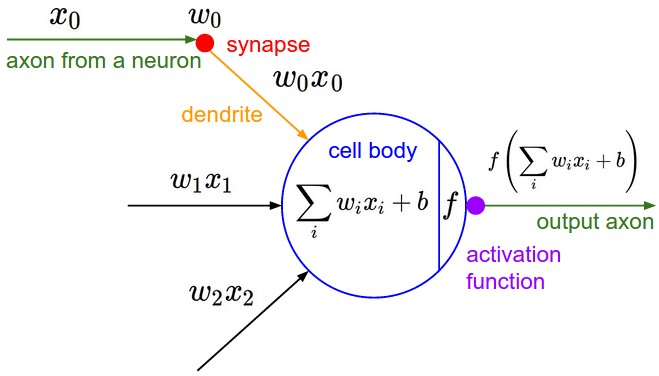
\includegraphics[scale=0.4]{neuron_model.jpeg}
\caption{Mô hình mạng neural}
\label{fig:splitdata}
\end{figure}
\end{itemize}
\item Kiến trúc mạng neural
\begin{itemize}
\item Mạng lan truyền tiến
\item Mạng hồi qui
\end{itemize}
\item 2 kiểu học trong mạng neural
\begin{itemize}
\item Học tham số: thay đổi tham số để thích nghi với dữ liệu và liên kết trong mạng 
\item Học cấu trúc: mục tiêu thay đổi cấu trúc thích nghi cấu trúc mạng 
\end{itemize}
\item Học tham số
\begin{itemize}
 \item Mỗi bước lặp học các trọng số w theo công thức: $w^t=w^t + \Delta w^{t}$
 \item $\Delta w^{t}=\eta r^tx^{t-1}$
 \item Với $\$eta$ là tốc độ học
 \item Để thuật toán hội tụ thì cần chọn tốc độ học thoả mãn:
 \begin{itemize}
 \item $\sum_{i=1}^na_n=\infty$
 \item $\sum_{i=1}^na_n^2<\infty$
 \end{itemize}
\end{itemize}
\end{itemize}
\subsection{Cài đặt}
\begin{itemize}
\item Số tầng ẩn: 2
\item Tâng ẩn 1: 2048 neural, tầng ẩn 2: 1024 neural
\item Hàm active: sigmod= $\frac{1}{1+e^{-x}}$
\item Hàm score: sigmod= $\frac{1}{1+e^{-x}}$
\item Hàm loss: $\frac{1}{2}\sum_{i=1}^n(y_i^2-p_i^2)<\infty$
\item Tốc độ học $\frac{1}{ \sqrt{n}} $
\item Giải thuật học : lan truyền ngược
\begin{itemize}
\item Công thức cập nhật tham số cho w tại tầng output: $\Delta w^{iq }=\eta \Upsilon_i out_q$
\item $\Upsilon_i=[y_i - p_i]f'(Net_i)$
\item Công thức cập nhật tham số cho tầng ẩn 1 và 2: $\Delta w^{qj}=\eta \Upsilon_q x_j$
\item $\Upsilon_q=f'(Net_q)\sum_{i=1}^n\Upsilon_i w_{iq}$
\end{itemize}
\item Ngôn ngữ lập trình: matlab
\end{itemize}
\subsection{Kết quả}
\begin{itemize}
\item Dữ liệu : 50000 bộ cho tập training, 10000 bộ cho tập test.
\item Phương pháp đánh giá: Hold out
\item Kết quả thu được 
\begin{itemize}
\item Thực nghiệm trên máy tính laptop core i5, tốc độ xử lý 
\item Chạy 7h với bộ xử lý Intel(R) Core(TM) i5CPU @ 2.60GHz - 3.0GHz
\item Độ chính xác$\approx 35 \%$  
\end{itemize}
\end{itemize}
\section{Convolutional Neural Networks(CNN)}
\subsection{Giới thiệu}
Convolutional Neural Networks tương tư như các mạng nerual network khác. Chúng được tạo thành từ các tế bào noron có thể học trọng số và biases.Mỗi noron thực hiện hiện môt số sản xuất và tùy chọn với đường phi tuyến.Toàn bộ mạng vẫn thể hiện một hàm số khả vi duy nhất: từ các điểm ảnh hình ảnh thô trên một đầu với điểm số lớp học khác. Chúng vẫn có một hàm lỗi(ví dụ như SVM/softmax) ở lớp cuỗi (với kết nối đầy đủ).
\subsection{Kiến trúc tổng quan CNN}
Mạng CNN có 4 tầng chính: Convolution Layer, ReLu Layer , Pooling Layer, Fully-Connected Layer.
\subsubsection{Lớp Convolution Layer (Conv)}
\begin{itemize}
\item[-] Nhận đầu vào là ma trận các điểm ảnh $(W_1*H_1*D_1)$ ($W_1*H_1$: kích thước của ảnh, $D_1$ số kênh màu (3 kênh màu nếu là ảnh màu đại diện cho 3 kênh màu (r,g,b))).
\item[-] Các tham số:
\begin{itemize}
\item[•] Số các filters K: Tham số chính của tâng Conv. Mỗi filter sẽ trượt qua ma trận đầu vào và đưa ra ma trận đầu ra. Mỗi filter là một ma trận có kích thước là tham số cần chọn, chiều của ma trận là chiều của ma trận đầu vào (trong bài toán này chiều của filter là 3 (số kênh màu)).
\item[•] Kích thước của mỗi filter F*F.
\item[•] Số ô nhat qua mỗi lần trượt.
\item[•] Zerro padding P: Tham số quyết định ma trận đầu vào và ma trận đầu ra có cùng kích thước không (có trượt hết tất cả các ô của ma trận đầu vào không hay nói cách khác là có trượt vượt ra khỏi ma trận đầu vào không).
\end{itemize}
\item[-] Đầu ra là ma trận kích thước $W_2*H_2*D_2$:
\begin{itemize}
\item[•] $W_2 = (W_1 - F + 2P)/S + 1$.
\item[•] $H_2 = (H_1 - F + 2P)/S + 1$.
\item[•] $D_2 = K$.
\end{itemize}
\end{itemize}
\subsubsection{Lớp RELU Layer}
Tầng sẽ áp dụng hàm tác động, thông thường sẽ làm hàm ReLu max(0,x).Hàm sẽ tác động lên từng phần tử của ma trận đầu vào nên ma trận đi qua tầng này sẽ không thay đổi kích thước.
\subsubsection{Lớp PoolingLayer}
\begin{itemize}
\item[-] Thường chèn tầng pooling vào giữa các tầng Conv để giảm kích thước ma trận.
\item[-] Nhận đầu vào là ma trận $W_1*H_1*D_1$ là kích thước của ma trận đầu ra của tầng Conv.
\item[-] Các tham số:
\begin{itemize}
\item[•] Kích thước của ma trận pooling $F*F$.
\item[•] Số ô nhảy qua sau mỗi lần trượt trên ma trận input.
\end{itemize}
\item[-] Đầu ra là mậ trận kích thước $W_2*H_2*D_1$.
\begin{itemize}
\item[•] $W_2 = \frac{(W_1 - F)}{S} + 1$.
\item[•] $H_2 = \frac{(H_1 - F)}{S} + 1$.
\item[•] $D_2 = D_1$.
\end{itemize}
\end{itemize}
\subsubsection{Lớp Fully-connected Layer}
\begin{itemize}
\item[-] Như mạng neuron thông thường,các neuron trong tầng Fully-connected kết nối với toàn bộ các neuron ở tầng trước nó: Nhận đầu vào là vector áp dụng hàm tác động và đưa ra đầu ra.
\end{itemize}
\begin{figure}[h]
\begin{center}
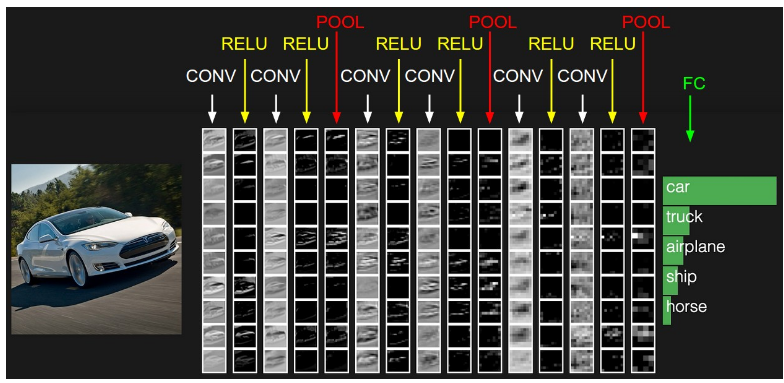
\includegraphics[width =0.8 \textwidth]{ConvNetArchitecture.png}
\end{center}
\end{figure}
\subsubsection{Lớp Max norm constraint và Dropout}
Để giảm overfit ta có thể áp dụng các kỹ thuật như:
\begin{itemize}
\item[-] Thêm max norm constraint cho các trọng số.
\begin{itemize}
\item[•] Khi cập nhật các trọng số thì các trường số phải thỏa mãn điều kiện: \\ 
 $\Vert\overrightarrow{w}\Vert_{2} < c$(c thường được chọn 3 hoặc 4). 
\end{itemize}
\item[-] Thêm tầng dropout
\begin{itemize}
\item[•] Đầu ra của các tầng trước tầng drop-out khi đi qua tầng drop-out sẽ được giữ nguyên với xác là p hoặc sẽ được chuyển thành 0 với xác suất 1-p.
\end{itemize} 
\end{itemize}
\subsection{Update tham số}
\subsubsection{Momentum update}
$\Delta w^{t+1} = \Delta w^{t} + \mu .\Delta w^{t} - \eta . \nabla E^t$.
\subsubsection{Nesterov momentum}
$w^{(t+1) = w^{t} + \mu . \Delta w^t}$ \\
$\Delta w^{(t+1)} = \mu . \Delta w^t - \eta . \nabla E^{t+1}$.
\begin{figure}[h]
\begin{center}
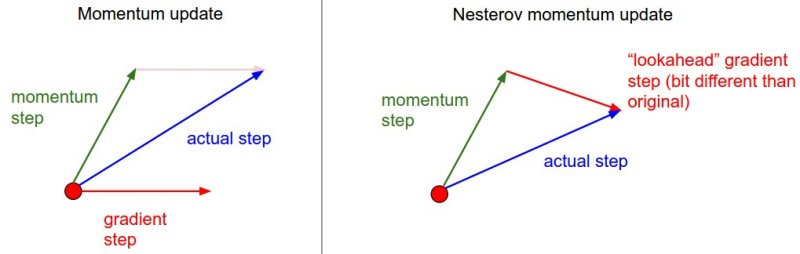
\includegraphics[width =0.8 \textwidth]{paramUpdate.jpeg}
\end{center}
\end{figure}
\subsection{Mạng CNN Đơn giản}
\subsubsection{Cấu trúc mạng}
\subsubsection{Cài đặt chương trình}
Sử dụng thư viện keras
\begin{itemize}
\item[-] Load data và xử lí dữ liệu:
\begin{lstlisting}
(X_train, y_train), (X_test, y_test) = cifar10.load_data()

# normalize inputs from 0-255 to 0.0-1.0
X_train = X_train.astype('float32')
X_test = X_test.astype('float32')
X_train = X_train / 255.0
X_test = X_test / 255.0


# one hot encode outputs
y_train = np_utils.to_categorical(y_train)
y_test = np_utils.to_categorical(y_test)
num_classes = y_test.shape[1]
\end{lstlisting}
\item[-] Thêm các tầng
{\small
\begin{lstlisting}
# Create the model
model = Sequential()
model.add(Convolution2D(32,3,3,input_shape=(3,32,32),... 
 	border_mode='same',activation='relu',...
 			W_constraint=maxnorm(3)))
model.add(Dropout(0.2))
model.add(Convolution2D(32,3,3,activation='relu',...
	border_mode='same',...
			W_constraint=maxnorm(3)))
model.add(MaxPooling2D(pool_size=(2, 2)))
model.add(Flatten())
model.add(Dense(512,activation='relu',...
		W_constraint=maxnorm(3)))
model.add(Dropout(0.5))
model.add(Dense(num_classes, activation='softmax'))
\end{lstlisting}
}
\begin{itemize}
\item[•] Các tầng Conv có các tham số:
\begin{itemize}
\item[*] Số filter: 32
\item[*] Kích thước mỗi filter: $3*3*3$.
\item[*] input\_shape: Nhận đầu vào là ma trận ảnh $32*32*3$.
\item[*] border\_mode: kích thước ma trận đầu vào và ma trận đầu ra là như nhau (32*32).
\item[*] W\_constraint: max norm constraint với c = 3.
\end{itemize}
\item[•] Sau mỗi tầng Conv là tầng ReLu
\item[•] Tầng Drop-out thứ nhất với xác suất chuyển các tham số về 0 là 0.2
\item[•] Tầng Pooling với fiter có kích thước 2*2
\item[•] Tầng Flattern để chuyển ma trận thành vector 
\item[•] Tầng Dense (Fully-connected):
\begin{itemize}
\item[*] Kích thước đầu ra: 512 (vector 512 chiều)
\item[*] Hàm tác động: relu
\item[*] W\_constraint:  max norm constraint với c = 3
\end{itemize}
\item[•] Tầng Drop-out thứ hai với xác suất chuyển các tham số về 0 là 0.2
\item[•] Tầng Dense (Fully-connected) cuối cùng:
\begin{itemize}
\item[*] Kích thước đầu ra: Số nhãn lớp (scroce cho mỗi nhàn lớp): 10 nhãn lớp
\item[*] Hàm tác động : softmax (vector x có n chiều) \\ \\ 
\hspace*{2cm} $\sigma(x_i) = \frac{e^{x_i}}{\Sigma_{j=1}^{n}e^{x_k}}$
\end{itemize}
\end{itemize}
\item[-] Traning:
\begin{lstlisting}
epochs = 25
lrate = 0.01
decay = lrate/epochs
sgd = SGD(lr=lrate, momentum=0.9, decay=decay, 
		nesterov=False)
model.compile(loss='categorical_crossentropy', 
			optimizer=sgd, metrics=['accuracy'])
print(model.summary())
# Fit the model
model.fit(X_train,y_train,validation_data=(X_test, y_test), 
			nb_epoch=epochs, batch_size=32)
\end{lstlisting}
\begin{itemize}
\item[•] Số epoch thực hiện 25
\item[•] Learning rate: 0.01
\item[•] Sử dụng minibatch gradient decent (số ảnh trong một batch là 32) với chiến lược tối ưu là momentum để update các tham số (tham số mu trong momentum là 0.9) không sử dụng nesterov momentum
\item[•] Hàm đánh giá lỗi: cross-entropy \\
\begin{center}
$L = -\frac{1}{N}\Sigma_{i=1}^{N}\big[y_i\log y_i + (1-\tilde{y_i})\big]$ (c là nhãn thực tế của ảnh i,$\tilde{y_i}$ là nhãn do mô hình dự đoán)
\end{center}
\end{itemize}
\end{itemize}
\subsubsection{Kết quả}
Độ chính xác: 71.26\%
\begin{figure}[H]
\begin{center}
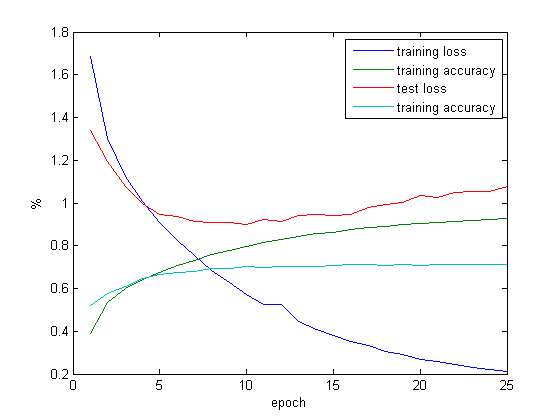
\includegraphics[width =1.0 \textwidth]{testImg.png}
\end{center}
\end{figure}
\subsection{Mạng CNN Lớn}
\subsubsection{Cấu trúc mạng}
{\small
$\textbf{INPUT} \rightarrow \textbf{CONV} \rightarrow \textbf{RELU} \rightarrow \textbf{DropOut} \rightarrow \big[\textbf{CONV} \rightarrow \textbf{RELU} \rightarrow \textbf{POOL\big]*2} \rightarrow \textbf{DropOut} \rightarrow \textbf{CONV} \rightarrow \textbf{RELU} \rightarrow \textbf{POOL} \rightarrow \textbf{FLatten} \big[\textbf{DropOut} \rightarrow \textbf{Fully-connect(RELU)\big]*2}\rightarrow \textbf{DropOut} \rightarrow \textbf{Ouput(num\_class,activation='softmax')}$
}
\newpage
{\small
\begin{center}
\begin{longtable}{lccl}
\caption{\textbf{Bảng mô tả mạng CNN}}
\label{}
\endfirsthead
\endhead
\hline
	Layer (type)              &      Output Shape     &     Param\#   &  Connected to  \\
\hline
convolution2d\_1 (Convolution2D) & (None, 32, 32, 32) &   896    &     convolution2d\_input\_1[0][0]     \\
\hline
dropout\_1 (Dropout)          &    (None, 32, 32, 32)  &  0     &      convolution2d\_1[0][0]            \\
\hline
convolution2d\_2 (Convolution2D)&  (None, 32, 32, 32) &   9248   &     dropout\_1[0][0]          \\        
\hline
maxpooling2d\_1 (MaxPooling2D)   & (None, 32, 16, 16)&    0       &    convolution2d\_2[0][0]      \\      
\hline
convolution2d\_3 (Convolution2D) & (None, 64, 16, 16) &   18496   &    maxpooling2d\_1[0][0] \\             
\hline
maxpooling2d\_2 (MaxPooling2D)   & (None, 64, 8, 8)    &  0        &   convolution2d\_3[0][0] \\
\hline
convolution2d\_4 (Convolution2D) & (None, 128, 8, 8)  &   73856   &    maxpooling2d\_2[0][0]      \\       
\hline
dropout\_2 (Dropout)  &            (None, 128, 8, 8) &    0   &        convolution2d\_4[0][0]       \\     

\hline
convolution2d\_5 (Convolution2D)&  (None, 128, 8, 8) &    147584 &     dropout\_2[0][0]            \\      

\hline
maxpooling2d\_3 (MaxPooling2D) &   (None, 128, 4, 4) &    0   &        convolution2d\_5[0][0]     \\       

\hline
flatten\_1 (Flatten)        &      (None, 2048) &         0    &       maxpooling2d\_3[0][0]    \\        

\hline
dropout\_3 (Dropout)    &          (None, 2048)  &        0   &        flatten\_1[0][0]    \\              

\hline
dense\_1 (Dense)      &            (None, 1024)     &     2098176   &  dropout\_3[0][0]    \\              

\hline
dropout\_4 (Dropout)  &            (None, 1024)  &        0  &         dense\_1[0][0]      \\              
\hline
dense\_2 (Dense)       &           (None, 512)  &         524800&      dropout\_4[0][0]        \\          

\hline
dropout\_5 (Dropout)    &          (None, 512) &          0      &     dense\_2[0][0]        \\           

\hline
dense\_3 (Dense)         &         (None, 10) &           5130    &    dropout\_5[0][0]          \\        

\hline
\end{longtable} 
\end{center}
}
Tổng params: 2878186
\subsubsection{Cài đặt chương trình}
Sử dụng thư viện keras,cài đặt tương tự với mạng CNN đơn giản với các tham số:
\begin{itemize}
\item[•] epochs = 25
\item[•] chiến lược tối ưu Stochastic gradient descent
\begin{itemize}
\item[-] Tỉ lệ học learn rate: lrate = 0.01
\item[-] decay = lrate/epochs
\end{itemize}
\end{itemize}
\subsubsection{Kết quả}
{\small
Epoch 1/25 \\
50000/50000 [===] - 1047s - loss: 1.8077 - acc: 0.3323 - val\_loss: 1.4027 - val\_acc: 0.4874 \\
Epoch 2/25 \\
50000/50000 [===] - 1034s - loss: 1.3529 - acc: 0.5107 - val\_loss: 1.2112 - val\_acc: 0.5600 \\
Epoch 3/25 \\
50000/50000 [===] - 1035s - loss: 1.1446 - acc: 0.5892 - val\_loss: 1.0184 - val\_acc: 0.6379 \\
Epoch 4/25 \\
50000/50000 [===] - 1034s - loss: 0.9922 - acc: 0.6457 - val\_loss: 0.9022 - val\_acc: 0.6826 \\
Epoch 5/25 \\
50000/50000 [===] - 1036s - loss: 0.8755 - acc: 0.6877 - val\_loss: 0.8355 - val\_acc: 0.7097 \\
Epoch 6/25 \\
50000/50000 [===] - 1036s - loss: 0.7894 - acc: 0.7218 - val\_loss: 0.7886 - val\_acc: 0.7226 \\
Epoch 7/25 \\
50000/50000 [===] - 1037s - loss: 0.7251 - acc: 0.7422 - val\_loss: 0.7389 - val\_acc: 0.7412 \\
Epoch 8/25 \\
50000/50000 [===] - 1036s - loss: 0.6710 - acc: 0.7617 - val\_loss: 0.7038 - val\_acc: 0.7522 \\
Epoch 9/25 \\
50000/50000 [===] - 1036s - loss: 0.6332 - acc: 0.7766 - val\_loss: 0.6907 - val\_acc: 0.7613 \\
Epoch 10/25 \\
50000/50000 [===] - 1037s - loss: 0.5886 - acc: 0.7902 - val\_loss: 0.6712 - val\_acc: 0.7712 \\
Epoch 11/25 \\
50000/50000 [===] - 1036s - loss: 0.5572 - acc: 0.8018 - val\_loss: 0.6407 - val\_acc: 0.7768 \\
Epoch 12/25 \\
50000/50000 [===] - 1036s - loss: 0.5205 - acc: 0.8163 - val\_loss: 0.6548 - val\_acc: 0.7731 \\
Epoch 13/25 \\
50000/50000 [===] - 1036s - loss: 0.4976 - acc: 0.8226 - val\_loss: 0.6613 - val\_acc: 0.7737 \\
Epoch 14/25 \\
50000/50000 [===] - 1036s - loss: 0.4705 - acc: 0.8332 - val\_loss: 0.6355 - val\_acc: 0.7869 \\
Epoch 15/25 \\
50000/50000 [===] - 1036s - loss: 0.4486 - acc: 0.8412 - val\_loss: 0.6241 - val\_acc: 0.7933 \\
Epoch 16/25 \\
50000/50000 [===] - 1041s - loss: 0.4310 - acc: 0.8475 - val\_loss: 0.6288 - val\_acc: 0.7886 \\
Epoch 17/25 \\
50000/50000 [===] - 1037s - loss: 0.4122 - acc: 0.8552 - val\_loss: 0.6321 - val\_acc: 0.7877 \\
Epoch 18/25 \\
50000/50000 [===] - 1037s - loss: 0.3932 - acc: 0.8608 - val\_loss: 0.6300 - val\_acc: 0.7916 \\
Epoch 19/25 \\
50000/50000 [===] - 1037s - loss: 0.3721 - acc: 0.8669 - val\_loss: 0.6214 - val\_acc: 0.7956 \\
Epoch 20/25 \\
50000/50000 [===] - 1038s - loss: 0.3561 - acc: 0.8729 - val\_loss: 0.6317 - val\_acc: 0.7929\\
Epoch 21/25 \\
50000/50000 [===] - 1037s - loss: 0.3448 - acc: 0.8765 - val\_loss: 0.6168 - val\_acc: 0.7987 \\
Epoch 22/25 \\
50000/50000 [===] - 1037s - loss: 0.3271 - acc: 0.8833 - val\_loss: 0.6551 - val\_acc: 0.7927\\
Epoch 23/25 \\
50000/50000 [===] - 1037s - loss: 0.3225 - acc: 0.8844 - val\_loss: 0.6334 - val\_acc: 0.7999 \\
Epoch 24/25 \\
50000/50000 [===] - 1037s - loss: 0.3071 - acc: 0.8895 - val\_loss: 0.6259 - val\_acc: 0.7993 \\
Epoch 25/25 \\
50000/50000 [===] - 1037s - loss: 0.2948 - acc: 0.8946 - val\_loss: 0.6318 - val\_acc: 0.7991 \\
}
\\
Trong đó:
\begin{itemize}
\item[•] loss: giá trị lỗi tập train
\item[•] acc:  giá trị chính xác
\item[•] val\_loss:  giá trị lỗi theo tập test
\item[•] val\_acc: giá trị lỗi theo tâp test
\end{itemize}
\subsubsection{Đồ thị biểu diễn}
\begin{figure}[h]
\begin{center}
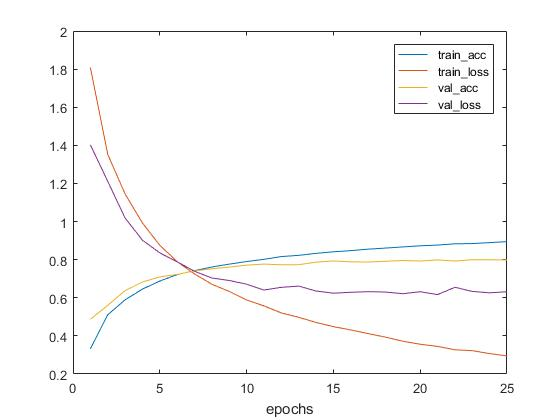
\includegraphics[width =1.0 \textwidth]{graph.png}
\end{center}
\end{figure}
\subsubsection{Thực nghiệm}
\begin{itemize}
\item[•] Train với bộ dữ liệu là 50000 mẫu và 10000 mẫu test.
\item[•] Sử dụng phương pháp đánh giá hand-out.
\begin{itemize}
\item[-] Dữ liệu được chia làm 2 phần tách biệt không giao nhau.
\item[-] Bộ dữ liệu với các ví dụ nhiễu lỗi ít
\end{itemize}
\item[•] Kết quả thu đươc:
\begin{itemize}
\item[-] Chạy 8h với bộ xử lý Intel(R) Core(TM) i5-3230M CPU @ 2.60GHz - 3.0GHz
\item[-] Chạy theo chiến lược min-batch(32).
\item[-] Độ chính xác khi đánh giá với tập test là: 79.91\%.
\end{itemize}
\end{itemize}
\section{SVM}
\subsection{Cơ sở lý thuyết SVM}
\subsubsection{Khái niệm-đặc điểm  }
SVM là một phương pháp phân lớp tuyến tính (linear
classifier), với mục đích xác định một siêu phẳng
(hyperplane) để phân tách hai lớp của dữ liệu.\\
SVM có một nền tảng lý thuyết chặt chẽ\\
SVM là một phương pháp tốt (phù hợp) đối với những bài
toán phân lớp có không gian rất nhiều chiều (các đối
tượng cần phân lớp được biểu diễn bởi một tập rất lớn
các thuộc tính)\\

Biểu đồ histogram:
Histogram là một dạng biểu đồ biểu diễn số lượng điểm ảnh tương ứng với mức độ sáng tối của bức ảnh.\\
\begin{figure}[H]
\centering
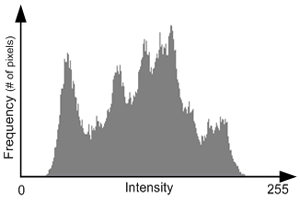
\includegraphics[scale=0.9]{histogram.png}
\caption{Histogram}
\label{fig:histogram}
\end{figure}
\subsection{Cơ sở lý thuyết}
Biểu diễn tập huấn luyện 
$${x_1, y_1}, (x_2,y_2),...(x_r,y_r)$$
\begin{itemize}
\item $x_i$ là một vectơ đầu vào $x_i \subseteq R^n$
\item $y_i\in{1,-1}$ là một nhãn lớp
Hàm phân tách tuyến tính 
$$f(x)=<w.x> +b$$
w là vectơ trọng số các thuộc tính, b là một giá trị số thực\\


\end{itemize}
\begin{figure}[H]
\centering
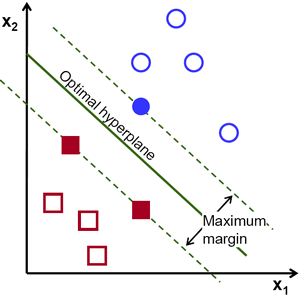
\includegraphics[scale=3.0]{margin-svm.png}
\caption{Siêu phẳng phân tách}
\label{fig:margin-svm}
\end{figure}
Khoảng cách từ một điểm đến siêu phẳng 
$$\frac{|<w.x_i>+b|}{||w||} $$
$$margin=d_+ +d_-=\frac{2}{||w||}$$ 
Tương đương bài toán cực tiểu hóa $\frac{<w.w>}{2}$ với điều kiện 
$$ \lbrace\begin{array}{l}
 <w.x_i>+b \geq 1 if y_i=1\\ <w.x_i>+b
    \leq -1  if y_i=-1 \end{array} $$
Áp dụng phương pháp Lagrange  
$$ L= 1/2 ||\overline{w}||^2 -\sum\alpha_i[y_i(\overline{w}.\overline{x_i} +b)-1] $$
Điều kiện 
$$ \frac{ \partial}{\partial\overline{w}}
=\overline{w}- \sum \alpha_i y_i x_i=0 \Longrightarrow \overline{w}=\sum \alpha_i y_i \overline{x_i} $$
$$\frac{ \partial}{\partial b}=-\sum \alpha_i y_i \Longrightarrow \sum x_i y_i=0$$ 
Thế vào ta được biểu thức :
$$L_D(\alpha)=\sum_{i=1}^r \alpha_i-1/2 \sum_{i,j=1}^{r}\alpha_i \alpha_j y_i y_j<x_i.x_j> $$
Điều kiện:
$$\{ \begin{array}{l}
\sum_{i=1 } ^{r} \alpha_i y_i =0 \\
\alpha_i \geq 0 \forall i=1..r
\end{array}
$$
Dung phương pháp lặp giải cuối cùng thu được
$$w^* =\sum_{x_i \in SV} \alpha_i y_i x_i  $$
$$b^*=y_k-<w*,x_k>$$
Để phân lớp cho giá trị mới ta tìm dấu của siêu phẳng $$ f(x)=\sum_{x_i \in SV} \alpha_i y_i <x_i .x>+b^*$$
Nới lỏng điểu kiện :
$$L_D(\alpha)=\sum_{i=1}^r \alpha_i-1/2 \sum_{i,j=1}^{r}\alpha_i \alpha_j y_i y_j<x_i.x_j> $$
$$
\{ \begin{array}{l}
\sum_{i=1 } ^{r} \alpha_i y_i =0 \\
0 \leq \alpha_i \leq C \forall i=1..r
\end{array}
$$
Phân lớp không tuyến tính một vài hàm nhân:\\
Đa thức $K(x,z)=(<x.z>+\Theta)^d $\\
Gaussian RBF $K(x,z)=e^{\frac{||x-z||^2}{2*\sigma}}$ trong đó $\sigma >0$\\
Phân lớp nhiều nhãn 2 chiến lược :
\begin{itemize}
\item one-versus-all
\item one-versus-one 
\end{itemize}
\subsection{Cài đặt áp dụng với bài toán phân loại ảnh}
\subsubsection{Công cụ}
Ngôn ngữ lập trình python, thư viện học máy scikit-learn, opencv
Đọc dữ liệu :
\begin{lstlisting}
#have 5 bacth 
#read batch 1
fo = open("data_batch_1", 'rb')
dict = cPickle.load(fo)
da=np.array(dict.get('data'))
lb=np.array(dict.get('labels'))
fo.close()
\end{lstlisting}
Huấn luyện mô hình kernel là hàm nhân sử dụng (rbf,linear,poly) C là tham số nới lỏng mô hình, gamma tham số ảnh của hàm nhân(ảnh hưởng đến giá trị).
Với hàm poly ta còn có tham số degree(mũ) và coef0(b) phương thức fit của SVC dùng để train mô hình 
\begin{lstlisting}
clf = SVC(C=5, kernel='rbf',gamma='auto')
from datetime import datetime
print("start",str(datetime.now()))
clf.fit(trainX, trainY)
print("end train",str(datetime.now()))
\end{lstlisting}
Đoán tập test: phương thức predict dùng để đoán nhãn cho tập test 
\begin{lstlisting}
res=clf.predict(testX)
print("end predict ",str(datetime.now()))
sol=(res==testY)
print(res[:10])
print(testY[:10])
print(sol[:10])
print(sol.sum())

\end{lstlisting}
Sử dụng histogram để xây dựng đầu vào cho SVM : 

Histogram với rbg color: sử dụng cv2 để tạo ra ma trận histogram , cv nhận đầu vào là ảnh nên ta phải chuyển ma trận từ dữ liệu thành ma trận ảnh rbg kích thước 32 32 3. \\
Các tham số của hàm  calcHist như sau 
\begin{itemize}
\item Đầu vào ảnh 
\item Số đại diện cho màu cần tạo histogram [0 1 2] tức là cả 3 màu r b g
\item bin tương ứng từng màu với dữ liệu ảnh theo (1) khuyên nên chọn 16 
\item Vùng màu chọn 
\end{itemize}
\begin{lstlisting}
lhistr=[]
for i in range(50000):
    #print i
    histr = cv2.calcHist(da[i].reshape((3,1024)).
    T.reshape((32,32,3)),[0,1,2 ],None,[16,16,16],[0,256,0,256,0,256])        
    lhistr.append(histr.ravel())

trainX=np.array(lhistr)
\end{lstlisting}
Histogram với gray color:
Sử dụng hàm chuyển đổi màu của opencv cvtColor() việc này đồng nghĩa sẽ giảm số chiều của dữ liệu xuống bằng bins ở đây là 16.
\begin{lstlisting}
lhistr=[]
for i in range(50000):
    #print i
    histr = cv2.calcHist(cv2.cvtColor(da[i].reshape((3,1024)).
    T.reshape((32,32,3)), cv2.COLOR_BGR2GRAY),[0],None,[16],[0,256])
    lhistr.append(histr.ravel())

trainX=np.array(lhistr)
\end{lstlisting}
Phương pháp đánh giá sử dụng: hold out
\subsection{Kết quả thực nghiệm}
Áp dụng toàn bộ với chiền lược one vs all
\begin{itemize}
\item SVM rbf C=5 autosklearn=(gamma=1/3072(xích ma=3072)) độ chính xác $\approx 25 \%$  
\item SVM poly C=5 autosklearn=(gamma=1/3072 n=3) độ chính xác $\approx 38,2 \%$
\item SVM linear C=5  độ chính xác $\approx 32 \%$    
\item SVM poly histogram bin=16 C=5 autosklearn=(gamma=1/3072 n=3) độ chính xác $\approx 37,6 \%$
\item SVM poly gray histogram bin=16 C=5 autoskcearn=(gamma=1/3072 n=3) độ chính xác $\approx 29,6 \%$
\end{itemize}
\chapter{Kết luận}
\section{So sánh các phương pháp}
\begin{enumerate}
\item Mạng CNN 79,91$\%$
\item SVM 38$\%$
\item Mạng neural(2 tầng) 35 $\%$
\item KNN 11$\%$
\end{enumerate}
Mạng CNN thể hiện là phương pháp khá ưu việt so với các phương pháp khác(79,91$\%$). \\Tiếp sau đó là SVM(38$\%$), mang neural(2 tầng) 35 $\%$ , KNN cuối cùng (11$\%$)
\section{Khó khăn gặp phải}
Phương pháp SVM
\begin{itemize}
\item Bộ dữ liệu lớn train rất lâu poly (5 tiếng) rbf(10 tiếng) rất khó để xử lý chọn các tham số 
\item SVM rất nhiều tham số cần phải thử nghiệm rất nhiều
\end{itemize}
Phương Pháp CNN
\begin{itemize}
\item Phần cứng chưa đủ mạnh trên dữ liệu lâu (6h - 8h).
\end{itemize}
Cách thức nhóm hoạt động:
\begin{itemize}
\item Xảy ra xung đột khi lập trình tổng hợp các phần code của các thành viên khi làm việc trên Git. \\
\textbf{Hướng giải quyết}: Nhóm dành thời gian tìm hiểu và thống nhất cách thức làm việc.

\item Khó khăn trong lịch hẹn gặp nhóm do thời gian biểu của từng thành viên trong nhóm là khác nhau.\\
\textbf{Hướng giải quyết}: Thảo luận trong nhóm online, chủ động sắp xếp thời gian để gặp mặt bàn bạc, có thể không được đầy đủ mọi thành viên cùng lúc nhưng cần đảm bảo thông tin đến các thành viên là đầy đủ và đúng lúc.


\end{itemize}
\section{Kinh nghiệm rút ra được}
\begin{itemize}
\item Tiếp cận với các công nghệ mới, đa dạng khả năng làm việc khi gặp vấn đề trong thực tế
\item Kỹ năng làm việc nhóm: Tích lũy thêm kinh nghiệm về cách thức trao đổi thông tin giữa các thành viên trong nhóm, tăng khả năng sử dụng các công cụ hỗ trợ làm việc nhóm như Github.
\item Tăng cường trao đổi online, tạo môi trường làm việc tích cực
\end{itemize}
\chapter{Tài liệu tham khảo}

\begin{verbatim}
[+] Slide Học Máy TS. Thân Quang Khoát
[+] Opencourse in Mit-SVM 
[+]  http://www.svm-tutorial.com/2016/09/unconstrained-minimization/
[+] https://ongxuanhong.wordpress.com/2015/09/19/support-vector-machine
-svm-hoi-gi-dap-nay/
[+] http://scikit-learn.org/stable/modules/generated/sklearn.svm.SVC.
html#sklearn.svm.SVC 
[+] SVMs for Histogram-Based Image Classification
Olivier Chapelle, Patrick Haffner and Vladimir Vapnik
[+] http://docs.opencv.org/3.1.0/d1/db7/tutorial_py_histogram_begins.html
[+] http://cs231n.github.io/convolutional-networks/
[+] https://keras.io/getting-started/sequential-model-guide/

\end{verbatim}


\end{document}
